% !TEX TS-program = pdflatexmk

%%%%%%%%%%%%%%%%%%%%%%%%%%%%%%%%%%%%%%%%%%%%%%%%%%%%%%%%%%%%%%%%%%
%%%%%%%% ICML 2016 EXAMPLE LATEX SUBMISSION FILE %%%%%%%%%%%%%%%%%
%%%%%%%%%%%%%%%%%%%%%%%%%%%%%%%%%%%%%%%%%%%%%%%%%%%%%%%%%%%%%%%%%%

% Use the following line _only_ if you're still using LaTeX 2.09.
%\documentstyle[icml2016,epsf,natbib]{article}
% If you rely on Latex2e packages, like most moden people use this:
\documentclass{article}

% use Times
\usepackage{times}
% For figures
\usepackage{graphicx} % more modern
%\usepackage{epsfig} % less modern
\usepackage{subfigure}

% For citations
\usepackage{natbib}

% For algorithms
\usepackage{algorithm}
\usepackage{algorithmic}

% As of 2011, we use the hyperref package to produce hyperlinks in the
% resulting PDF.  If this breaks your system, please commend out the
% following usepackage line and replace \usepackage{icml2016} with
% \usepackage[nohyperref]{icml2016} above.
\usepackage{hyperref}

% Packages hyperref and algorithmic misbehave sometimes.  We can fix
% this with the following command.
\newcommand{\theHalgorithm}{\arabic{algorithm}}

% Employ the following version of the ``usepackage'' statement for
% submitting the draft version of the paper for review.  This will set
% the note in the first column to ``Under review.  Do not distribute.''
\usepackage{icml2016}

% Employ this version of the ``usepackage'' statement after the paper has
% been accepted, when creating the final version.  This will set the
% note in the first column to ``Proceedings of the...''
%\usepackage[accepted]{icml2016}


\usepackage{amsthm}
\usepackage{amssymb}
\usepackage{amsmath}

% The \icmltitle you define below is probably too long as a header.
% Therefore, a short form for the running title is supplied here:
\icmltitlerunning{Particle Thompson Sampling for Knowledge Base Completion}

\begin{document}

\twocolumn[
\icmltitle{Particle Thompson Sampling for Knowledge Base Completion}

% It is OKAY to include author information, even for blind
% submissions: the style file will automatically remove it for you
% unless you've provided the [accepted] option to the icml2016
% package.
\icmlauthor{Your Name}{email@yourdomain.edu}
\icmladdress{Your Fantastic Institute,
            314159 Pi St., Palo Alto, CA 94306 USA}
\icmlauthor{Your CoAuthor's Name}{email@coauthordomain.edu}
\icmladdress{Their Fantastic Institute,
            27182 Exp St., Toronto, ON M6H 2T1 CANADA}

% You may provide any keywords that you
% find helpful for describing your paper; these are used to populate
% the "keywords" metadata in the PDF but will not be shown in the document
\icmlkeywords{machine learning, ICML}

\vskip 0.3in
]


%!TEX root = ./cikm2016.tex
\begin{abstract}
Knowledge base construction consists of two tasks: extracting information from external resources  (knowledge population) and inferring missing information through a statistical analysis on the extracted information (knowledge completion). 
In many cases, a lack of sufficient external resources in the knowledge population hinders the following statistical inference.
The gap between these two processes can be reduced by an incremental population approach via labelling of human experts.
We propose a new probabilistic knowledge base factorisation method that benefits from the path structure of existing knowledge (e.g. syllogism) and enables a common modelling approach to be used for both incremental population and knowledge completion tasks.
More specifically, the probabilistic formulation allows us to develop an incremental population algorithm that trades off exploitation-exploration.
Experiments on three benchmark dataset shows that the balanced exploitation-exploration helps the incremental population, and the additional path structure helps to predict missing information in the knowledge completion.
\end{abstract}

%!TEX root = ./cikm2016.tex

\section{Introduction}
\label{sec:intro}

Relational knowledge bases structuralise our understanding about the world into the form of \textit{(entity1, relation, entity2)} triples
that help reasoning and inferring in a wide range of tasks such as information retrieval, question answering, and semantic parsing~\cite{Dong2015,jiang2015improving,kim2013context,sondhi2014mining}.
A construction of a knowledge base is a very active research area with many important and challenging research questions.
The early stage of knowledge base construction relies on {\bf knowledge population} task
in which structured information from external sources are extracted, 
or human experts encode a prior knowledge manually.
Despite the endeavour toward to construct a complete knowledge base, 
even the commercialised knowledge bases are still far from complete~\cite{dong2014knowledge}. 
{\bf Knowledge completion} task has been emerged as an complement of the knowledge population 
to scale up the knowledge base construction. Unlike the knowledge population task where the goal is to maximise the number of triples, the goal of knowledge completion is to maximise the predictive performance on unseen triples through a statistical analysis on the extracted information \cite{guu2015traversing,Lao2010}.
%There are two main knowledge completion approaches. First, latent feature models factorise entities and relations to predict unseen triples. Second, graph feature models 

One major obstacle of knowledge base construction is a gap between knowledge 
population and completion. For example, when there is no external source to extract knowledge,
the construction relies solely on the contribution of human experts.
Manual labelling is often painful and tedious, 
therefore triples that will be labelled should be selected in an active way so 
that we can maximise the performance of following knowledge completion.
Active learning may provide a systematic way of selecting a data point to be labelled with one of knowledge completion models~\cite{Settles2010}. However, it is not clear that which model from the knowledge completion should be used for the active selection because of the discrepancy between two different goals of knowledge population and completion.
%However, the selection of proper model is still ambiguous and arbitrary for the active acquisition task. 
%In the active learning literature, it is often ignored that which model for a predictive task is appropriate for its active counterpart. 

We provide a model based active query selection approach to see how the models from the latter task can be used for the former task. We first reformulate a bilinear tensor factorisation~\cite{nickel2015review} in a probabilistic way, where entities and relations are embedded into latent feature space. And then we propose a novel tensor factorisation model that incorporates the graph structure of knowledge base into the factorisation model. These two probabilistic models provide a natural way of embracing uncertainty of triples that is crucial to develop 
an active triple selection for the active knowledge population.
With Thompson sampling~\cite{scott10bandit} -- an approach for solving the multi-armed bandit problem,
the model find an optimal trade-off between exploration and exploitation when identifying new triples.

Based on experiments with three real-world datasets, we find that the models outperformed in the knowledge completion may not perform well in the active knowledge population. Because, for the knowledge completion, it is important to find a better latent structure given current observation, for the active population, however, it is more important to  measure the uncertainty of a current model in order to explore the latent space efficiently over time.
As far as we know, this is the first study that explicitly reveals how the knowledge completion models result in different conclusions in the active knowledge population.

The contributions of this paper can be summarised as follows:
\begin{itemize}
\item We propose a probabilistic reformulation of bilinear tensor factorisation that allows us to predict and measure the uncertainty of unobserved triples in Section \ref{sec:brescal}.
\item We incorporate a compositional structure of knowledge graph into the proposed factorisation by modelling a composition of relations as an algebraic operation in the probabilistic embedding space in Section \ref{sec:comp}.
\item We propose an active knowledge population method that efficiently explore the factorised space guided by a principled way of exploration-exploitation via Thompson sampling algorithm in Section \ref{sec:pts}.
\item Experiments on the knowledge completion with three real-world dataset show that the compositional model predicts unseen triples better than the bilinear factorisation model in Section \ref{sec:exp1}.
\item Experiments show the importance of uncertainty in the active population. Especially, the better predictive model does not guarantee to have a better knowledge population due to an improper uncertainty measure in Section \ref{sec:exp2}.
\end{itemize}

\eat{
%KG background from text, completion
Relational knowledge bases support reasoning, information retrieval, 
or question-answering tasks about entities and their relations.
Most of them contain facts in the form of (entity1, relation, entity2) triples, 
such as (CarlFriedrichGauss, BornIn, Braunschweig).
%(ThomasBayes, London, BornIn).
Automatically acquiring, maintaining, and reasoning in
knowledge bases is a very active topic area with many important and challenging research questions. 
%, has sustained attention from both academia and industry. 
Even the largest of such databases are known to be incomplete~\cite{dong2014knowledge}. %min2013distant
There are two main ways to fill in the missing facts:
the first learning new relations from large collections of text or hyper-text,
%~\cite{Mintz2009,carlson2010toward}, 
known as knowledge extraction, 
the second is inferring facts from existing relations, %~\cite{Lao2010,nickel2015review} 
known as knowledge completion. 

%There are two open 
One challenge in knowledge base completion is 
its disconnection from the knowledge extraction setting. 
It would be nice, for example, to know which question to query for in 
a search-based method for gathering triples~\cite{west2014knowledge}. 
Recently \cite{kajino2015active} propose an active learning strategy for completing 
knowledge triples; however the algorithm had problems simultaneously achieving high recall and faithful reconstruction.
% finds it difficult to achieve 
%high recall and high reconstruction at the same time. 
Having an active exploit-explore strategy would more effectively 
connect knowledge completion and extraction problems. 
Another challenge is leveraging compositional knowledge from existing triples. 
Also known as paths in knowledge graphs, composition of facts is key to 
achieving common reasoning tasks. 
For example, the two triples (CarlFriedrichGauss, BornIn, Braunschweig)
and (Braunschweig, LocatedIn, Germany) implies (CarlFriedrichGauss, BornIn Germany). 
Path ranking~\cite{Lao2010}, vector space traversal~\cite{guu2015traversing}
and composition~\cite{Neelakantan2015} techniques 
are recently developed to leverage such information for knowledge completion. 
We note, however, that a principled formulation that can address 
both open challenges is still missing -- namely, a relational model 
that can model knowledge compositions in an active setting. 

%\TODO{TODO}{revise summary-of-our-approach to be consistent w. the above}
We propose a novel probabilistic reformulation of tensor factorisation,  
one of the main competitive variants for knowledge completion~\cite{nickel2015review}. 
%There are many advantages to a probabilistic formulation of tensor factorisation, 
%such as the quantification of uncertainty by the predictive distribution, 
%the ability to utilise priors, and the availability of principled model selection. 
We name our model probabilistic RESCAL (PRESCAL).
The probabilistic model provides a natural way of 
embracing uncertainty of triples that is crucial to develop 
%implementing
an active triple selection for knowledge completion, using  
Thompson sampling~\cite{scott10bandit} -- an approach for solving the multi-armed bandit problem,
which allows us to trade-off exploration and exploitation when identifying new triples.
%randomized probability matching, also known as Thompson sampling~\cite{scott10bandit}.
We also perform compositional training for the probabilistic model, 
by modeling relation compositions as algebraic operations in the probabilistic embedding space. 
For inference, we design Gibbs sampling for PRESCAL with and without compositions. 
%with by computing conditional posteriors. 
We employ a sequential Monte-Carlo method for the active querying of new triples, 
called particle Thompson sampling. 

We first test the proposed models with synthetic datasets. 
We observe that Thompson sampling provides significant gain over random sampling of triples; 
we also observe a clear gain in tensors with known composition structure. 
We then evaluated the model on three real-world relation datasets. In the passive learning setting, 
we find PRESCAL outperforming the non-probabilistic version of tensor factorisation, 
and that compositions help when the training set is sparse. 
In the active learning scenario, 
we find that PRESCAL achieves the highest cumulative gain across all datasets. 
It is encouraging to see the exploitation-exploration strategy with uncertainty outperforming 
active learning strategies that focus solely on exploitation or exploration. 

We are pleased to be able to learn a vector-space model for entities and relations with uncertainty, 
bridging the gap of probabilistic active sampling and knowledge compositions. 
We look forward to follow-on work with better sampling strategies and computational scalability. 
}

\eat{
Statistical relational models have been proposed to tackle
various problems of knowledge bases. For example, it can be used 
for question understanding and answering problems ,
or it can be integrated into a search engine
to improve the users' search experiment \cite{dong2014knowledge}.

However, most of previous latent feature models lack the consideration
of constructing a knowledge graph with the latent features.
As an alternative approach, distant supervision algorithms
\cite{Mintz2009} suggest a way to fill a missing part of knowledge graph
through the extensive NLP processing, however, this method inherently
requires a set of initial observations used as a distant supervision.

Here, we tackle the problem of knowledge base construction with the
statistical relational model.
A goal of knowledge base construction is to acquire a maximum number
of valid triples with a limited budget.
This goal corresponds to a general objective of the multi-armed bandit (MAP)
problem where we want to minimise the cumulative regret or maximise
the cumulative reward over time. 
In recent years, Thompson sampling has been emerged as  
an competitive solution in MAP problems.
We borrow Thompson sampling, which provides a principled
way to find an optimal trade off between exploration and exploitation,
to solve the knowledge base construction problem.
}

\eat{
We propose a compositional relation model that exploit the compositional structure of 
knowledge graph to capture the latent semantic structure of the entities and relations.
While previously suggested vector space models provide a statistical way to infer the latent semantic 
structure of entities and relations, but lack consideration of a graph structure of a knowledge base itself.

In a separate way from the vector space models, graph feature algorithms such as the path ranking algorithm 
are suggested to fill a missing part of a knowledge graph \cite{Lao2010}. The graph feature algorithms 
directly include graph structures, such as edge type, node type, and node degree, to learn and predict new 
triples, however, the absence of latent structure makes the models failed to predict a new triple when the 
target entities does not have rich structural background\cite{nickel2015review}.

We propose a compositional vector space model that benefits the latent representation of vector space model 
along with the graph structure of the graph feature models. Recently, Guu et. al. suggest a compositional 
training framework for vector space models \cite{gu2015traversing}, where paths over a knowledge graph act 
as a new form of structural regularisation of the models. Based on their work, we extend the compositional 
approach within a probabilistic framework with two compositional structures.
}

\eat{%% v1 of intro
As the amount of information codified in a computer readable fashion increases, the management
of knowledge bases need to become increasingly more automated. In this paper, we study
the problem of acquiring new knowledge given an existing knowledge base. Knowledge bases
are modelled as a set of relations between pairs of entities, for example the factoid
``Barack Obama is the 44th president of the United States''
is modelled as two entities (Barack Obama, United States) being related by ``president of''.
Such relations have a natural representation as a sparse graph or a tensor of order 3.
Given this representation, we model the acquisition of new knowledge as the
identification of new triples that capture particular relations between two entities.

There are several challenges when we apply machine learning methods to completing
existing knowledge bases, namely:
sparse, noisy, and incomplete annotations.
There has been recent success in transferring ideas from matrix completion problems to
the tensor domain to overcome the challenge of sparsity~\cite{unknown}.
We follow this thread of research by using a low rank approximation model for tensor
factorisation. Such low rank approximations can also be seen as a latent variable probabilistic
model, which additionally captures the inherent uncertainty of noisy annotations.
We propose a probabilistic model for tensor factorisation and explore both the Gaussian
and Logistic model. The probabilistic model provides a natural way of implementing
randomised probability matching, also known as Thompson sampling~\cite{scott10bandit}.
Thompson sampling is an approach for solving the multi-armed bandit problem,
which allows us to trade off exploration and exploitation when identifying new triples.
This provides a principled approach to identify promising candidates for knowledge base
completion.
We additionally consider compositional relations as an additional source of weak information
to further utilise the existing (incomplete) knowledge items.

Goal of this paper 1: Populating knowledge graph with an active label acquisition process 
corresponding to [B,C,A] in Figure \ref{fig:related3d}.

[B,C,P] could be an alternative direction (or both).
}

%!TEX root = ./icml2016.tex

\section{Related Work}

\begin{figure}[t]
	\centering
	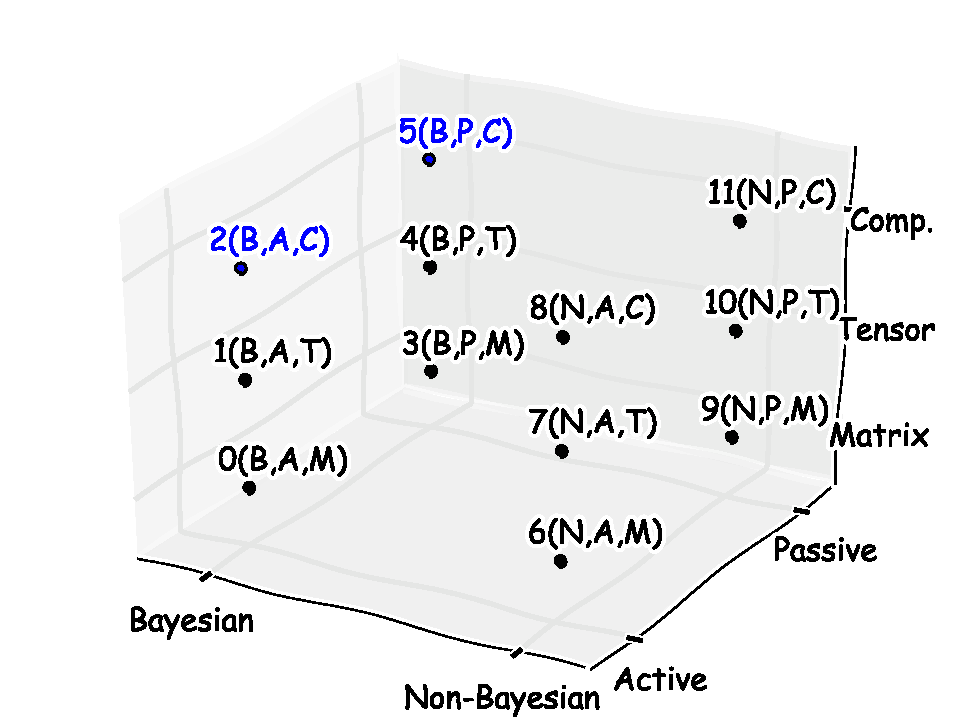
\includegraphics[width=\linewidth]{images/3d_plot.pdf}			
	\caption{\label{fig:related3d}Scope of our work}
\end{figure}

\begin{itemize}
\item [B,A,M] Efficient Thompson Sampling for OnlineMatrix-Factorization Recommendation\cite{kawale2015efficient}. Active learning and search on low-rank matrices \cite{sutherland2013active}. Collaborative filtering as multi armed bandit \cite{guillou2015collaborative}
\item [N,A,M] Matrix completion with queries \cite{ruchansky2015matrix}.
\item [B,P,M] PMF \cite{mnih2007probabilistic} ...
\item [N,P,M] NMF\cite{lee1999learning} ...
\item [B,P,T] Bayesian Tensor Factorisation models. CANDECOMP/PARAFAC (CP) decomposition \cite{xiong2010temporal,schmidt2009probabilistic}, CP and TUCKER3 \cite{yilmaz2012algorithms}
\item [N,A,T] Populating knowledge graph with active learning (IBM) \cite{kajino2015active}
\item [N,P,T] Rescal \cite{nickel2011three}, TransE \cite{bordes2013translating}, and many others.
\item [N,P,C] Compositional vector space model \cite{Neelakantan2015}, 
\end{itemize}

Might be relevant, but not positioned in the figure.
\begin{itemize}
\item Clustering based Bayesian approach for learning relations: Infinite relational model based on entity clustering \cite{kemp2006learning}.
\item Path ranking algorithm (graph feature model) \cite{Lao2010}
\end{itemize}

%!TEX root = ./cikm2016.tex
\section{Probabilistic RESCAL}
\label{sec:brescal}

\begin{table*}[bt]
\caption{Parameters for Gibbs updates. The conditional posterior of $e_i$ and $R_k$ follows the normal distribution with mean $\mu$ and precision matrix $\Lambda$. $\otimes$ is the Kronecker product.}
\label{tab:brescalposterior}
\vskip 0.05in
\begin{tabu}{l|l|l|l}
var&$\mu$&$\Lambda$&$\xi$\\
\hline
$e_i$&
$\frac{1}{\sigma_x^2}\Lambda_i^{-1}\xi_i$&
$\frac{1}{\sigma_x^2} \sum_{jk : x_{ikj} \in \mathcal{X}^{t}} (R_k e_j)(R_k e_j)^\top$&
$\sum_{jk : x_{ikj} \in \mathcal{X}^{t}}  x_{ikj} R_{k} e_{j} +
\sum_{jk : x_{jki} \in \mathcal{X}^{t}} x_{jki} R_{k}^\top e_{j}.$
\\
$vec(R_k)$&
$\frac{1}{\sigma_x^2}\Lambda_k^{-1}\xi_k$&
$\frac{1}{\sigma_x^2} \sum_{ij:x_{ikj} \in \mathcal{X}^{t}} (e_i
\otimes e_j)(e_i \otimes e_j)^\top + \frac{1}{\sigma_r^2} {I}_{D^2}$&
$\sum_{ij:x_{ikj} \in \mathcal{X}^{t}} x_{ikj} (e_{i} \otimes e_{j}).$
\end{tabu}
\end{table*}


A relational knowledge base consists of a set triples in the form of $(i, k, j)$
where $i$, $j$ are entities, and $k$ is a relation. A triple can be distinguished
in a valid triple and invalid triple based on a semantic meaning of a triple. An
example of valid triple in Freebase is (BarackObama, PresidentOf, U.S.), and an
example of invalid triple is (BarackObama, PresidentOf, U.K.).
A knowledge base can be represented in a three-way binary tensor
$\mathcal{X} \in \{0, 1\}^{N \times K \times N}$, where $K$ is a number of
relations, $N$ is a number of entities, and $x_{ikj}\in\mathcal{X}$ indicates whether
the triple is valid.

We model the entities $i$ as vectors $e_i$ and the relations $k$ as matrices $R_k$ with an
appropriately chosen latent dimension $D$. This follows a popular model
for statistical relational learning, which is to factorise the tensor into a
set of latent vector representations, such as the bilinear model RESCAL~\cite{nickel2011three}.
RESCAL aims to factorise each relational slice $X_{:k:}$ into a set of rank-$D$ latent
features as follows:
\[
  \mathcal{X}_{:k:} \approx E R_k E^\top, \qquad \text{for } k = 1, \dots, K
\]
Here, $E\in {\mathbb R}^{N \times D}$ contains the latent features of the
entities $e_1, \ldots, e_N$ and $R_k\in {\mathbb R}^{D \times D}$ models the interaction of the
latent features between entities in relation $k$.

We propose a probabilistic framework that directly generalises RESCAL
by placing priors over the
latent features. For each entity $i$, the latent feature of an entity $e_i \in
\mathbb{R}^{D}$ is drawn from an isotropic multivariate-normal distribution.
\begin{align}
\label{eqn:entity_gen}
e_i \sim {N}(\mathbf{0}, \sigma_e^2{I}_D)
\end{align}
For each relation $k$, we draw matrix $R_k$ from
a zero-mean isotropic matrix normal distribution.
\begin{align}
\label{eqn:relation_gen}
R_k \sim \mathcal{MN}_{D \times D}(\mathbf{0}, \sigma_r{I}_D, \sigma_r{I}_D) \\
\text{or equivalently}\enspace r_k  = \text{vec}(R_k) \sim N(\mathbf{0}, \sigma_r^2 I_{D^2}) \notag
\end{align}
where $\text{vec}(R_k)$ denotes the flattening of the matrix.

We consider two observation models for $x_{ikj}$: a real or random variable. By placing a
normal distribution over $x_{ikj}$,
\begin{align}
  x_{ikj} |e_i, e_j, R_k \sim \mathcal{N}(e_i^{\top} R_k e_j, \sigma_x^2) \label{eqn:triple_gen}
\end{align}
we can control the confidence on different observations
through the variance parameter $\sigma_x^2$.
The role of this parameter will be further discussed in the compositional model section.

We develop an efficient Gibbs sampler to perform inference for the probabilistic RESCAL (PPRESCAL).
The key for achieving efficiency are the two conditional posteriors for latent features.
The Gibbs updates are given by:
\begin{align}
p(e_i |E_{-i}, \mathcal{R}, \mathcal{X}^{t}, \sigma_e, \sigma_x) &= \mathcal{N}(e_i | \mu_i,
\Lambda_i^{-1})  \label{eqn:sample_e} \\
p(R_k|E, \mathcal{X}, \sigma_r, \sigma_x) &= \mathcal{N}(\text{vec}(R_k) |
\mu_k, \Lambda_k^{-1}) \label{eqn:sample_r}
\end{align}
where the negative subscript $-i$ indicates the every other entity variables except $e_i$.
The means and precision matrices are listed in Table~\ref{tab:brescalposterior}, where we have
used the identity $e_i^{\top} R_k e_j = r_k^{\top} e_i \otimes e_j$.

Alternatively, we may want to more precisely model the fact that the observations are binary.
Therefore we model $x_{ikj}$ as a binomial distributed random variable whose
probability is determined by logistic regression.
\[
p(x_{ikj}=1) = \sigma(e_i^{\top} R_k e_j),
\]
where $\sigma$ is a sigmoid function.
We approximate the conditional posterior of
$E$ and $R$ by Laplace approximation~\cite{bishop2006pattern}. The maximum a
posterior estimate of $e_i$ or $R_k$ given the rest can be computed through the
standard logistic regression solvers with regularisation parameters as the priors over $e_i$ and $R_k$. Given the
maximum a posteriori parameters $e_i^*$, the posterior covariance $S_i$ of entity
$i$ takes the form
\begin{align*}
S_i^{-1} = \sum_{x_{ikj}} \sigma(e_{i}^{*\top} R_k e_{j}) (1 - \sigma(e_{i}^{*\top} R_k e_{j})) R_k
e_{j}(R_k e_{j})^\top\\
 + \sum_{x_{jki}} \sigma(e_{j}^{\top} R_k e_{i}^*) ( 1- \sigma(e_{j}^{\top} R_k e_{i}^*)) R_k^\top e^*_{i}(R_k^\top e^*_{i})^\top + I\sigma_e^{-1}
.
\end{align*}
The posterior covariance of $R_k$ can be computed in the same way, and is shown in the appendix.

There are many advantages to a probabilistic view of tensor factorisation, such as
the quantification of uncertainty by the predictive distribution,
the ability to utilise priors, and
the availability of principled model selection.
We show in the empirical experiments that PRESCAL outperforms standard RESCAL.
In the following, we focus on the predictive distribution, which enables us to
improve sequential knowledge acquisition.

%!TEX root = ./icml2016.tex
\section{Particle Thompson Sampling}

Thompson sampling has been gaining an increasing attention
because of a competitive empirical performance as well as its conceptual
simplicity~\cite{scott10bandit,li11thompson}. Let $y_{1:t}$ be a sequence of rewards up to time $t$, and $\theta$ is an underlying parameter governing the rewards. With Thompson sampling, an agent choose action $a$ according to its probability of being optimal:
\begin{align}
\arg\max_a \int \mathbb{I}\bigg[ \mathbb{E}(r|a, \theta)
= \max_{a'}\mathbb{E}(r|a',\theta) \bigg] p(\theta|y_{1:t-1}) d\theta, \notag
\end{align}
where $\mathbb{I}$ is an indicator function. Note that it is sufficient
to draw a random sample from the posterior instead computing the integral.

We formulate Thompson sampling for knowledge base construction
system as follows.
First, we assume there are optimal latent features $E^*$ and $R^*$, and
the triples are generated through Equation \ref{eqn:entity_gen}$-$
\ref{eqn:triple_gen}. At time $t$, the system draws samples $E^t$ and $R^t$
from the posterior distribution, and then chooses an optimal triple $(i,k,j)^*
= \arg\max_{i,k,j} e_i^\top R_k e_j$ to be queried. Finally, with the newly
observed triple $x_{(i,k,j)^*}$, the system updates the posterior of the latent
features.

The main difficulty of applying Thompson sampling to this task is a sequential update of the posterior distribution of the latent features with new observations over time. Unlike the point estimation algorithms such as
the maximum likelihood estimate, computing a full posterior with MCMC
requires extensive computational cost. To make the algorithm feasible, we employ a sequential Monte-Carlo (SMC) method for online posterior inference, generalising an algorithm proposed
in~\cite{kawale2015efficient} to tensors.

The SMC starts with $H$ number of particles, each of which starts with likelihood
weight $w_{h} = 1/H$, and a set of randomly sampled latent features $E^{h_0}$ and $R^{h_0}$.
With a slight abuse of notation, let $\mathcal{X}^{t}$ be a set of observed triples up to time $t$.
At time $t$, the system chooses one particle according to the particle weights,
and then generates a new query via Thompson sampling from the selected particle.
After observing a new variable, the system updates the posterior samples of
every particle through the MCMC kernels with the new observation.
We first sample the relation matrices using Equation \ref{eqn:sample_r}, and sample the entity vectors using Equation \ref{eqn:sample_e}.
Under the mild assumption where
$p(\Theta | \mathcal{X}^{t-1}) \approx p(\Theta | \mathcal{X}^{t})$,
the weight of each particle at time $t$ can be computed as follows
\cite{del2006sequential,chopin2002sequential}:
\begin{align}
w_{h}^{t} = \frac{p(\mathcal{X}^{t} | \Theta)}{p(\mathcal{X}^{t-1} | \Theta)}
 = p(x^{t} | \Theta, \mathcal{X}^{t-1})
\end{align}
To keep the posterior samples
on regions of high probability mass, we resample the particles whenever
an effective sample size (ESS) is less than a predefined threshold.
The ESS can be computed as $(\sum_h w_h^2)^{-1}$, and we set the threshold
to $N/2$ \cite{Doucet2011}. Resampling removes low weight particles with high probability,
while keeping samples from the posterior.
We summarise the particle Thompson sampling for Bayesian RESCAL with the
Gaussian output variable in Algorithm \ref{alg:smc}.

We show that the Thompson sampling approach improves over passive Bayesian RESCAL in
experiments with real and synthetic data.
We also investigated the extension of the Rao-Blackwellisation approach as proposed
in~\cite{kawale2015efficient}, but we did not observe any significant performance improvements.
We describe our extension in the appendix.

%\subsection{(?)Particle Thompson sampling with SGLD kernel}
%Above two algorithms are not well suitable for large scale dataset because the sample requires quantities estimated over all possible triples.
%
%Is it possible to use the stochastic gradient Langevin dynamics (SGLD) \cite{welling2011bayesian} kernel $K(E' | E)$ to sample $E'$ given $E$ with or without auxiliary variable $R_k$?
%\begin{align}
%e_i' \leftarrow e_i + \frac{\epsilon_t}{2}\Bigg\{\nabla \log p(\mathcal{X}|e_i) + \nabla \log p(e_i|\sigma_e)\Bigg\} + \nu_t
%\end{align}
%where, $\nu_t \sim \mathcal{N}(0, \epsilon_t I)$.

\begin{algorithm}[t!]
   \caption{Particle Thompson sampling for Bayesian RESCAL with Gaussian output variable}
   \label{alg:smc}
\begin{algorithmic}
   \STATE {\bfseries Input:} $\mathcal{X}^{0}, \sigma_x, \sigma_e, \sigma_r$.
   \FOR{$t=1,2, \dots$}
   \STATE \textit{Thompson Sampling}:
   \STATE $h_t \sim $ Cat$(\mathbf{w}^{t-1})$
   \STATE $(i,k,j) \leftarrow \arg\max p(x_{ikj}| E^{h_{t-1}}, \mathcal{R}^{h_{t-1}})$
   \STATE Query $(i,k,j)$ and observe $x_{ikj}$
   \STATE $\mathcal{X}^{t} \leftarrow \mathcal{X}^{t-1} \cup \{x_{ikj}\}$

   \STATE \textit{Particle Filtering}:
   \STATE $\forall h, w_h^{t} \propto p(x_{ikj} | E^{h}, \mathcal{R}^{h})$   \hfill $\triangleright$ Reweighting
   \IF{ESS$(\mathbf{w}^{t}) \leq N$}
   \STATE resample particles
   \STATE $w_h^{t} \leftarrow 1/H$
   \ENDIF

   \FOR{$h=1$ {\bfseries to} $H$}
   \STATE $\forall k, R_k^{h_t} \sim p(R_k | \mathcal{X}^{t}, E^{h_{t-1}}, R_{-k})$   \hfill $\triangleright$ see Table (\ref{tab:brescalposterior})
   \STATE $\forall i, e^{h_t}_i \sim p(e_i | \mathcal{X}^{t}, E_{-i}, \mathcal{R}^{h_{t}})$ \hfill $\triangleright$ see Table (\ref{tab:brescalposterior})
   \ENDFOR

   \ENDFOR
\end{algorithmic}
\end{algorithm}

%!TEX root = ./icml2016.tex
\section{Compositional Relations}


In this section, we propose a compositional relation model that exploit the compositional structure of
knowledge graph to capture the latent semantic structure of the entities and relations.
While previously suggested vector space models provide a statistical way to infer the latent semantic
structure of entities and relations, but lack consideration of a graph structure of a knowledge base itself.
%%LX: the above para is also in intro right now.

The compositionality represents a semantic meaning of a path over a knowledge graph that corresponds to a
sequence of composable triples.
For example, given two triples, ``Barack Obama is a 44th president of U.S.'' (Barack Obama / president of /
U.S) and ``Joe Biden was a running mate of Barack Obama'' (Joe Biden / running mate of / Barack Obama),
one can naturally deduce that the ``Joe Biden is a vice president of U.S.'' (Joe Biden / vice president of / U.S.).
Here the composition of two relations, president of, and running mate of, yield to a compositional relation,
vice president of.
% Is every running mate always a vice president? maybe this is not a proper example.
More formally, if there is a sequence of triples where the target entity of a former triple is a source entity of a
latter triple in a consecutive pair of triples in the sequence, then we can form a compositional triples
as follows.
Given the sequence of triples
$(i_1, k_1 ,j_1)$,  $(i_2, k_2, j_2)$, $(i_2, k_2, j_2)$ $\dots$ $(i_n, k_n, j_n)$, where $i_k = j_{k+1}$ for all $k
$,  we form a compositional triple $(i_1, {c}(k_1, k_2, \dots, k_n), j_n)$, where $c$ denotes the compositional
relation of the sequence of relations.

Let $\mathcal{C}^{L}$ be a set of all possible compositions of which length is up to $L$, $c \in \mathcal{C}$
be a sequence of relations, $c(i)$ be $i$th index of a relation in sequence $c$ and $|c|$ be the length of the
sequence. With set of compositions $\mathcal{C}^{L}$, we can expand set of observed triples
$\mathcal{X}^{t}$ to set of compositional triples $\mathcal{X}^{\mathcal{C}^{L}(t)}$ in which
compositional triple $x_{icj}$ is an
indicator variable that show the existence of the path from entity $i$ to entity $j$ through sequence
of relations
$c$ in $\mathcal{X}^{t}$. Note that the compositional relation $c$ is an abstract relation, and there might be a
multiple possible paths from $i_1$ to $j_n$.

With these extended compositional triples, we again model $x_{icj}$ with a bilinear Gaussian distribution,
\begin{align}
x_{(i, {{c}(k_1, k_2)}, l)} \sim \mathcal{N}(e_i^\top R_{{c}(k_1,k_2)} e_j, \sigma_{c}^2),
\end{align}
where $R_{{c}(k_1,k_2)} \in \mathbb{R}^{D\times D}$ is a latent matrix of compositional relation $c$, and $
\sigma_{c}^2$ is a covariance of the compositional triples. We keep the same latent vector $e$ for each entity
to model both normal triples and compositional triples.
In the subsequent sections, we provide two different ways of modelling the compositional relation $R_c$.

\subsection{Additive Compositionality}
First, we define an additive compositional relation $R_c$ as a sequence of normalized summation over
relation matrices in composition $c$, i.e.,
$R_{{c}} = \frac{1}{|c|}(R_{c(1)} + R_{c(2)} + \dots + R_{c(|c|)})$, then compositional triple $x_{icj}$
is modeled as
\begin{align}
x_{(i, c, j)} &\sim \mathcal{N}(e_i^\top R_c e_j, \sigma_{c}^2) \\
&= \mathcal{N}(e_i^\top \frac{1}{|c|}(R_{c(1)} + R_{c(2)} + \dots + R_{c(|c|)}) e_j, \sigma_{c}^2). \notag
\end{align}
The conditional distribution of $e_i$ given $E_{-i}, \mathcal{R}, \mathcal{X}^{t}, \mathcal{X}^{L(t)}$ is
expanded from the posterior of BRESCAL by incorporating compositional triples.
\begin{align} \label{eqn:comp_sample_e}
p(e_i |E_{-i}, \mathcal{R}, \mathcal{X}^{t}, \mathcal{X}^{L(t)}) &= \mathcal{N}(e_i | \mu_i, \Lambda_i^{-1}).
\end{align}

To compute the conditional distribution of $R_k$, we first decompose $R_c$ into two part where $R_c =
\frac{1}{|c|} R_k + \frac{|c|-1}{|c|}R_{c/k}$, where $R_{c/k} = \sum_{k' \in c/k} R_{k'}$.
The distribution of compositional triple is decomposed as follows:
\begin{align}
x_{(i, c, l)} \sim \mathcal{N}(e_i^\top (\frac{1}{|c|} R_k + \frac{|c|-1}{|c|}R_{c/k}) e_j, \sigma_{c}^2).
\end{align}
Then, the conditional distribution $R_k$ given $R_{-k}, E, \mathcal{X}^{t}, \mathcal{X}^{L(t)}$ is
\begin{align}
\label{eqn:comp_cond_r}
p(R_k|E, \mathcal{X}^{t}, \mathcal{X}^{L(t)}, \sigma_r, \sigma_x)  &= \mathcal{N}(\text{vec}(R_k) | \mu_k,
\Lambda_k^{-1}).
\end{align}

The mean and precision are obtained by expanding out the sum across $\mathcal{X}^{t}$ and
$\mathcal{X}^{L(t)}$. The details of the parameters are shown in the appendix.


\subsection{Multiplicative Compositionality}
Second, we define an multiplicative compositional relation $R_c$ as a sequence of multiplication over
relations in composition $c$, i.e. $R_c = R_{c(1)} R_{c(2)} \dots R_{c(|c|)}$, and the compositional triple as a
bilinear Gaussian distribution with the compositional relation $R_c$,
\begin{align}
x_{(i, c, j)} \sim \mathcal{N}(e_i^\top R_{c(1)}R_{c(2)} \dots R_{c(|c|-1)}R_{c(|c|)} e_j, \sigma_{c}^2)
\end{align}
The multiplicative compositionality can be understood as a sequence of linear transformation from the original
entity $i$ with the compositional relations, and the inner product between the transformed entity and target
entity will form a value of the compositional triple.

Given a sequence of relations including relation $k$, $R_k$ is placed in the middle of the compositional
sequence, i.e., $e_i^\top R_{c(1)}R_{c(2)} \dots R_{c(\delta_k)} \dots R_{c(|c|-1)}R_{c(|c|)} e_j$, where $
\delta_k$ is the index of relation $k$. For notational simplicity, we will denote the left side $e_i^\top R_{c(1)}
R_{c(2)} \dots R_{c(\delta_k -1)}$ as $\bar{e}_{ic(:\delta_k)}^\top$, and the right side $R_{c(\delta_k + 1)} \dots
R_{c(|c|-1)}R_{c(|c|)} e_j$ as $\bar{e}_{ic(\delta_k:)}$, therefore we can rewrite the mean parameter as $
\bar{e}_{ic(:\delta_k)}^\top R_{k} \bar{e}_{ic(\delta_k:)}$. With the simplified notations, the conditional of $R_k$
is
\begin{align}
p(R_k|E, \mathcal{X}, \sigma_r, \sigma_x)  &= \mathcal{N}(\text{vec}(R_k) | \mu_k, \Lambda_k^{-1}),
\end{align}
where
the mean and precision are obtained by expanding out the product across $\mathcal{X}^{t}$ and
$\mathcal{X}^{L(t)}$. The details of the parameters are shown in the appendix.
The conditional distribution of $e_i$ given the rest is the same as Equation $\ref{eqn:sample_e}$.

As the length of sequence $c$ increases, a small error in the first few multiplication will result a large
differences in the final compositional relation. One way to mitigate the cascading error is to increase variance
of compositional triples $\sigma_c$ as the length of the sequence increases.

%If the determinant of latent relation $R_k$ is greater than 1, the compositional latent relation $R_c$ might
%be exploded after multiplying a long sequence of relations. To obtain a stable scale of compositional
%relation $R_c$, one may multiply decaying factor $\tau < 1$ after each composition. $R_c = \tau^{|c|-1}
%R_{c(1)} R_{c(2)} \dots R_{c(|c|)}$.

%!TEX root = ./icml2016.tex
\section{Experiments}

In this section, we 
\rev{show results for Thomson sampling and compositions for BRESCAL. 
First on two synthetic datasets, and then on three common benchmarks for knowledge graphs.}
\eat{verify the Thompson sampling for Bayesian RESCAL (BRESCAL) 
through a synthetic dataset, and show how the active knowledge acquisition using Thompson sampling benefits the balance between exploitation and exploration
to compare with the exploitation only algorithms. And then, we show how the compositional model
improves the non-compositional models for finding a latent vector representation of knowledge bases.
}\rev{These experiments compare exploitation and exploration
 with exploitation only algorithms, and also show how the compositional model
improves the entity embedding upon the non-compositional models. }
%%LX: second sentence can be cut if we need space.

\eat{
In this section, we verify the Thompson sampling for Bayesian RESCAL (BRESCAL) 
through the synthetic dataset. We fit the compositional model in general
passive learning settings and show how the compositionality helps to find the 
latent features.
And then, we show how the active knowledge acquisition using Thompson sampling 
benefits the balance between exploitation and exploration to compare with the 
exploitation only algorithms. 
>>>>>>> bd7f11cb775339cba3a538a6f68351c2251ea530
}

\subsection{\rev{Thompson Sampling on }synthetic data}
\begin{figure}[t]
	\centering
	\subfigure[\scriptsize Logistic: N=10, K=10, D=5\label{fig:syn1}]{
	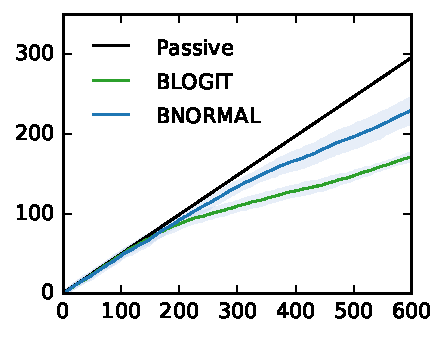
\includegraphics[width=0.42\linewidth]{images/toy_logit_vs_normal_10_10_5.pdf}
	}
	\subfigure[\scriptsize Logistic: N=20, K=10, D=5\label{fig:syn2}]{
	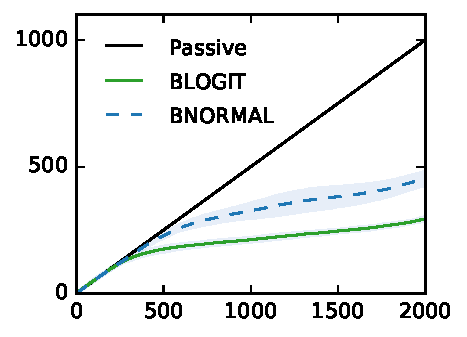
\includegraphics[width=0.445\linewidth]{images/toy_logit_vs_normal_20_10_5.pdf}
	}
	\subfigure[\scriptsize Gaussian: N=10, K=10, D=5\label{fig:syn3}]{
	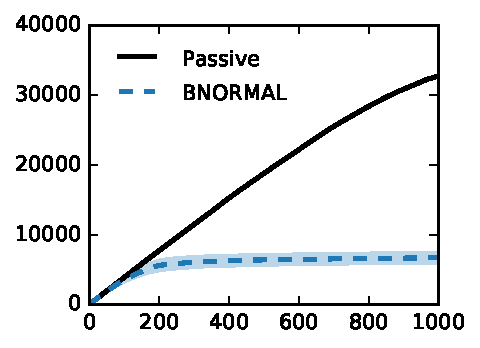
\includegraphics[width=0.42\linewidth]{images/toy_10_10_5.pdf}
	}
	\subfigure[\scriptsize Gaussian: N=20, K=10, D=5\label{fig:syn4}]{
	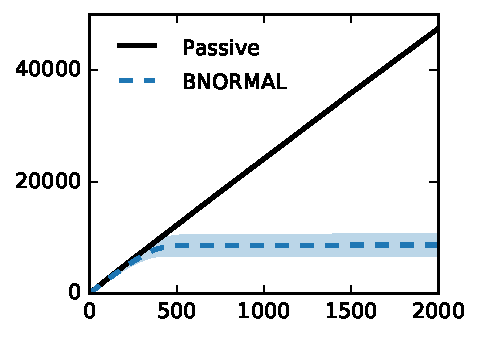
\includegraphics[width=0.45\linewidth]{images/toy_20_10_5.pdf}				
	}
%	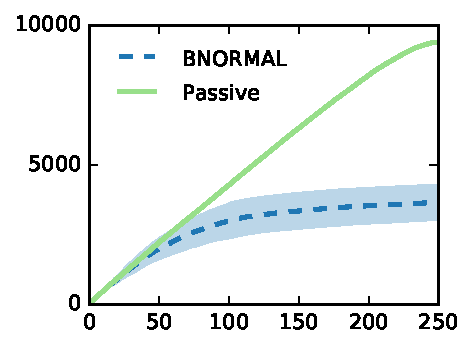
\includegraphics[width=0.32\linewidth]{images/toy_5_10_5.pdf}			
%	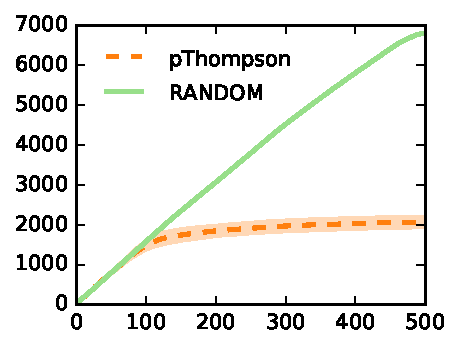
\includegraphics[width=0.32\linewidth]{images/toy_10_5_5.pdf}				
	\caption{\label{fig:synthetic} Cumulative regret of particle Thompson sampling with Gaussian and logistic output ({\sc BNORMAL, BLOGIT}) against Passive learning 
	on synthetic datasets with logistic	(top row, a, b) and Gaussian (bottom row, c, d) output variables.
	%We compared the particle Thompson sampling with passive sampling method. 
	The averaged cumulative regrets over 10 runs are plotted with one standard error. 
	As the model obtained more and more labeled samples from Thompson sampling, 
	the cumulative regrets increase sub-linearly.}
\end{figure}

\eat{To verify the particle Thompson sampling, }We first synthesise two \eat{sets of }datasets 
\eat{based on the model assumptions and run the Thompson sampling algorithm. By }
following the model assumptions in Eq. \ref{eqn:entity_gen} to 
\verify{\ref{eqn:triple_gen}}. 
\eat{We randomly generate triples based on randomly sampled entities and relations. Every }
\rev{First, }entities and relations are generated from zero-mean isotropic multivariate normal distribution, \eat{where we set }\rev{with } 
variance parameters $\sigma_e=1$, $\sigma_r=1$, respectively.
\rev{We generate two sets of \eat{the final}output triples,}
\eat{we generate two sets of datasets with }
\rev{with} the logistic output \eat{output variable }and the Gaussian \rev{with $\sigma_x$ set to 0.1}\eat{ variable}, respectively (Sec~\ref{sec:brescal}). 
\eat{The variance of gaussian $\sigma_x$ set to 0.1.}

To measure performance\eat{ on synthetic dataset}, we compute cumulative regret 
\eat{of proposed algorithm }at each time $n$ as $R(n) = \sum_{t=1}^{n} x_t - x^{*}_t$, 
%\begin{align}
%R(n) = \sum_{t=1}^{n} x_t - x^{*}_t,
%\end{align}
where $x^*_t$ is the highest\rev{-valued} triple among triples that have not been chosen up to time $t$. Unlike the general 
bandit setting where one can select a single item multiple times, in our formulation, we can select one triple 
only once. So after selecting a triple at time $t$, the selected triple will be removed from a set of candidate 
triples.

Figure \ref{fig:synthetic} shows the cumulative regret of the algorithm on the synthetic data with varying size of 
entities and relations. We compare the cumulative regret of the particle Thompson sampling with the passive 
learning method where the model choose a random triple at each time. All results are averaged over 10 
individual runs with different initialisations. 
Note that the dataset with binary logistic output variables can be used to train both Bayesian logistic RESCAL (BLOGIT) and Bayesian Gaussian RESCAL (BNORMAL) whereas the dataset with the Gaussian output can only be trained by BNORMAL.
Figure \ref{fig:syn1} and \ref{fig:syn2} show that with the logistic synthetic dataset both models are capable to learn the latent features of the generated triples, with logistic out-performing the Gaussian; Figure \ref{fig:syn3} and \ref{fig:syn4} show that BNORMAL \rev{out-perform passive learning in} the real valued dataset. 
%For every experiment, the cumulative regret of the Thompson 
%sampling method was bounded after a certain number of interactions whereas the cumulative regret of 
%passive learning increases linearly. 
\eat{Both results indicate the particle sampling is capable of inferring latent features 
of entities and relations as the interaction increases.}

\subsection{Thompson sampling for compositional models on synthetic data}
\begin{figure}[t]
	\centering
	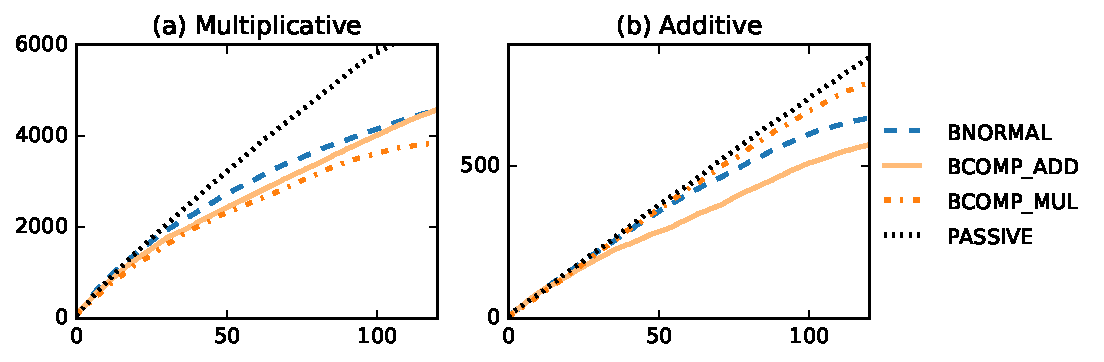
\includegraphics[width=\linewidth]{images/toy_comp_5_2_5.pdf}
	\caption{\label{fig:comp_synthetic} Cumulative regret of particle Thompson sampling of the compositional models on synthetic dataset with N=5, D=5. The synthetic dataset has three relations (K=3); the first two are independently generated, and the third relation is composed by the first two relations. The dataset used in (a) is generated by the multiplicative assumption, and the dataset used in (b) is generated by the additive assumption.}
\end{figure}

We conduct a second experiment on synthetic dataset to measure the 
performance of the Thompson sampling for the compositional models.
As in the first experiment, we first generate entities and relations from 
zero-mean multivariate normal with variance parameter $\sigma_e = 1$ and 
$\sigma_r=1$. We generate a set of triples with Gaussian output as in 
Eq. \ref{eqn:triple_gen}. We then synthesise two sets of expanded tensors 
using the previously used entities and relations based on the multiplicative 
and additive compositional assumptions, defined in Sec \ref{sec:comp}, 
respectively. So we synthesise fully observable expanded tensor $\mathcal{X}^L$ 
where $L=2$. We set both variance parameter $\sigma_x$ and $\sigma_c$ to 0.1.

To run the particle Thompson sampling on the synthetic dataset, we let the 
compositional models know which relation is composed by other relations. 
However, the BRESCAL model assumes each relation is independent to one another. 
Therefore, the compositional model uses much less number of parameters to model 
the same size of tensor to compare with the non-compositional model. 
\eat{%%LX: these info repeats?
Through 
this experiments, we verify the particle Thompson sampling algorithm for the 
compositional models.

For the experiment, we generate three relations ($K=3$) of five entities ($N=5$): 
the first and second relations 
are independent and the third relation is composed by the first and second 
relations. The latent dimension is set to 5.
}
With this fully observable expanded tensors, we run the Thompson sampling of 
the compositional models.
Figure \ref{fig:comp_synthetic} shows the cumulative regrets on synthetic 
datasets. The multiplicative and additive compositionality are used to 
generate the dataset for Figure \ref{fig:comp_synthetic}(a) and 
\ref{fig:comp_synthetic}(b), respectively. The results correspond to our 
assumption: the multiplicative compositional model (BCOMP-MUL) shows lower 
regrets on the multiplicative data in Figure \ref{fig:comp_synthetic}(a), and 
the additive compositional model (BCOMP-ADD) shows lower regrets on the 
additive compositional data in Figure \ref{fig:comp_synthetic}(b), 
and both have lower regrets than passive learning or BNORMAL with no composition. 

\subsection{Training compositional model on real datasets}
We evaluate the compositional models on three benchmark datasets and compare the performance to various baseline 
algorithms. We use three relational datasets: KINSHIP, UMLS, and NATION. Detailed description of each 
dataset is shown in Table \ref{tbl:dataset} \footnote{https://alchemy.cs.washington.edu/papers/kok07/}.

\begin{table}[t]
\centering
\caption{\label{tbl:dataset}Description of datasets. 
Sparsity denotes the ration of valid triples to invalid triples.}
\vskip 0.15in
\begin{tabular}{l | r | r | r | r}
Dataset &  \# rel & \# entities & \# triples & sparsity \\ \hline
Kinship & 26 & 104  & 10,790 & 0.038 \\
UMLS & 49 &135  & 6,752 & 0.008 \\
Nation & 56 & 14  & 2,024 & 0.184 \\
%Wordnet & 11 & 38,696  &123,429 & 7.5e-06\\
%Wordnet(N) & 10 & 836 & 1,766 & 2.5e-04\\
\end{tabular}
\end{table}


\begin{figure}[t]
	\centering
	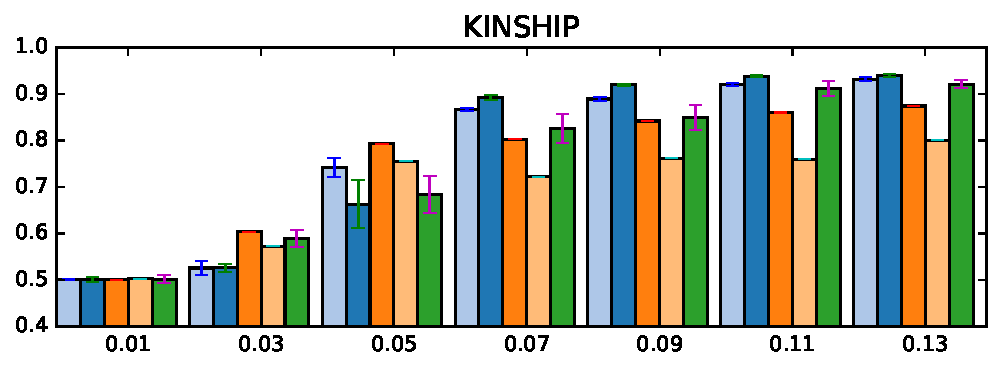
\includegraphics[width=\linewidth]{images/comp_training_error_kinship_small.pdf}
	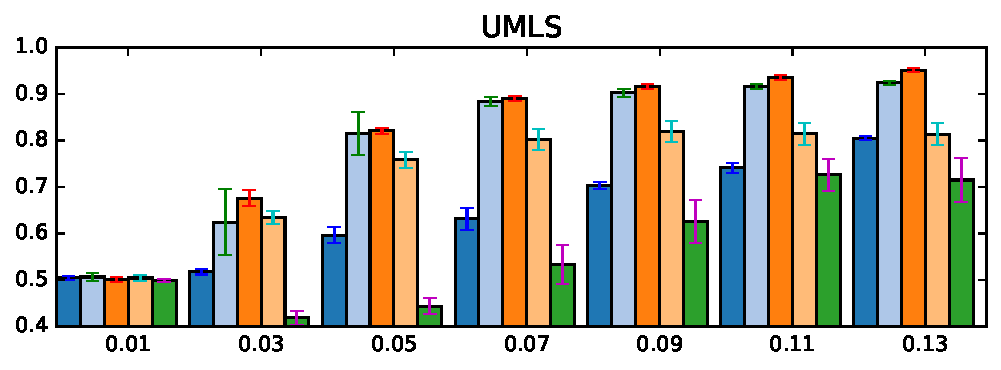
\includegraphics[width=\linewidth]{images/comp_training_error_umls_small.pdf}			
	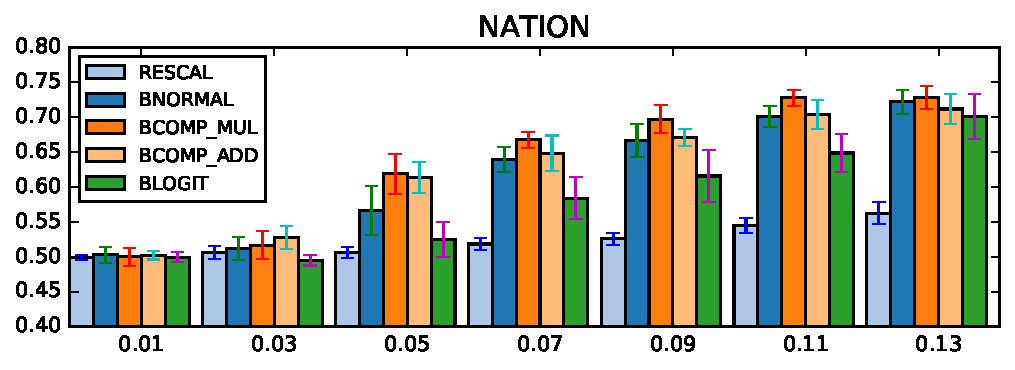
\includegraphics[width=\linewidth]{images/comp_training_error_nation_small.pdf}				
	\caption{\label{fig:r_vs_br} ROC-AUC scores of compositional models. 
	The x-axis denotes the proportion of an observed triples including negative triples used for training 
	models. %We use other 20\% of triples as a validation set and another 30\% of triples as a test set. 
}
\end{figure} 

%Applying Thompson sampling to the compositional models is not straight forward. 
%Because, in the compositional model, adding one valid triple in a knowledge base will 
%change the accompanying compositional paths over the extended tensor $\mathcal{X}^L$. 
%Therefore, the system requires to compute potential changes in the 
%compositional structure for every candidate query triple. This computational complexity 
%will increase exponentially as we increase the length of the composition.

%In this experiment, instead running the Thompson sampling for the compositional models,
We first evaluate our model in a non-active setting, 
%we follow the standard train/validation/test approach 
to measure the performance of BRESCAL with all non-compositional and compositional variants.
%The results between active acquisition and training and testing are not always coincident, but if the Thompson sampling samples latent features from true posterior of the compositional model, the samples corresponds to the true posterior samples from the training set.

For all experiments, we set the compositional length $L$ to 2, split the dataset into 20\% for validation and 30\% for testing. We vary the proportion of training triples
from 1\% to 13\% of datasets. For RESCAL, we use the authors' implementation, and measure performance over 10 runs with random initialisations. For BRESCAL and all the variants, we sample triples $x_{ikj}$ from its posterior, and measure performance over 10 different samples.
%Based on the trained model, measure the ROC-AUC scores on the test set.

Figure \ref{fig:r_vs_br} shows the ROC-AUC scores of the compositional models with the various baseline models. We can see that BNORMAL or BLOGIT generally out-perform RESCAL. We compare the compositional model with original RESCAL, BNORMAL, and BLOGIT. In general, BCOMP-MUL out-performs BCOMP-ADD, and performs better the other baseline models when the proportion of training set is small. For UMLS and NATION, BCOMP-MUL out-performs across the all training proportions. For KINSHIP, however, the model performs better when the training proportion is less than 7\%.


\subsection{Thompson sampling on real datasets}

\begin{figure*}[t]
	\centering
	
	\subfigure[KINSHIP]{
	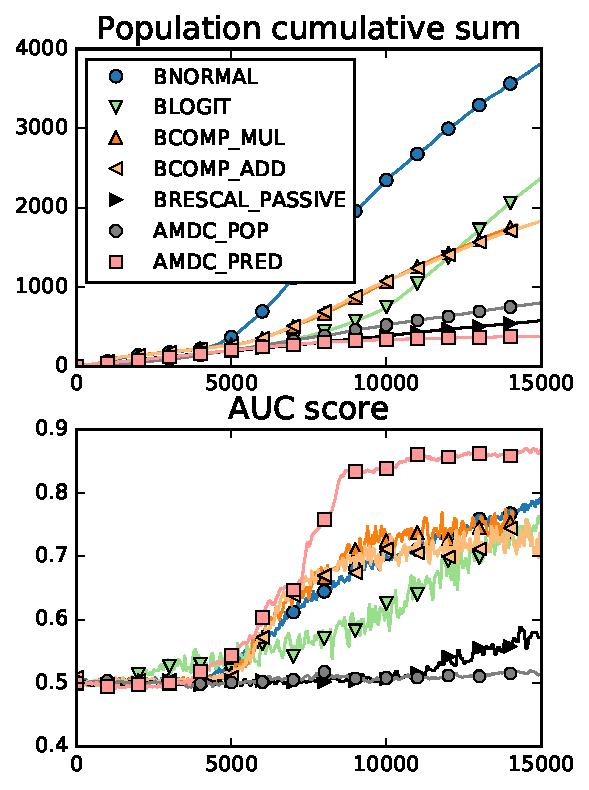
\includegraphics[width=0.3\linewidth]{images/thompson_kinship_vertical.pdf}
	}
	\subfigure[UMLS]{
	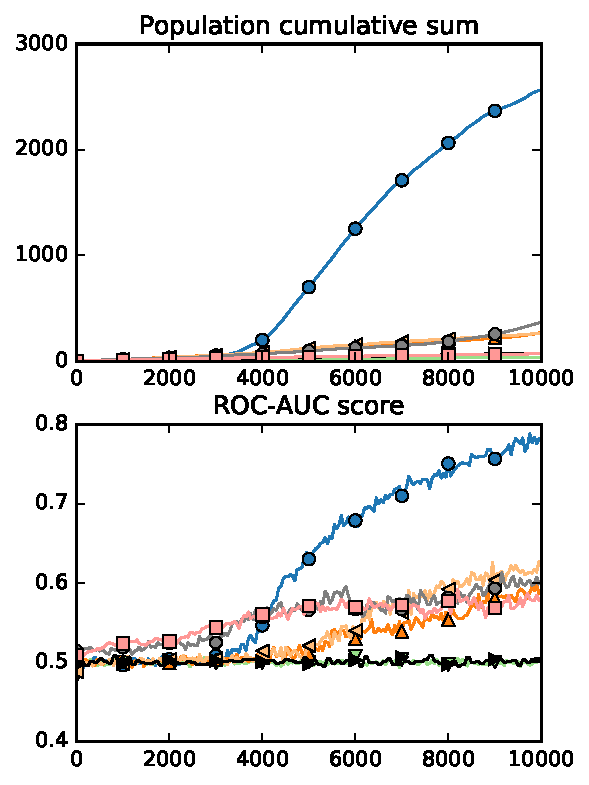
\includegraphics[width=0.3\linewidth]{images/thompson_umls_vertical.pdf}				
	}
	\subfigure[NATION]{
	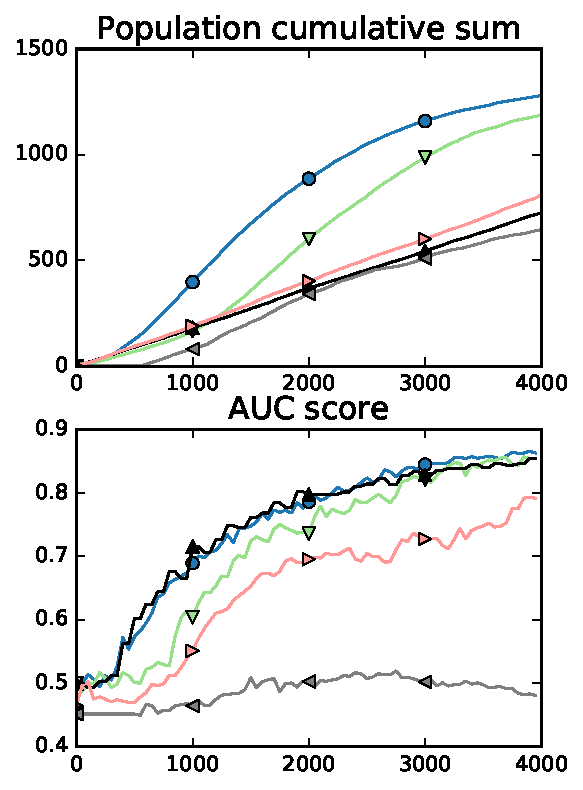
\includegraphics[width=0.3\linewidth]{images/thompson_nation_vertical.pdf}				
	}	
	\caption{\label{fig:c_gain}The cumulative gain and ROC-AUC score of the Thompson sampling 
	with various baseline approaches. Thompson sampling with Bayesian RESCAL (BNORMAL)
	model achieves the highest cumulative gain to compare with other active and 
	passive learning algorithms and shows comparable performance on ROC-AUC scores.}
\end{figure*}

Next, we evaluate the Thompson sampling for both compositional and non-compositional models on real datasets.

\textbf{Experimental settings}: 
We compare our model with AMDC, and passive learning with BRESCAL.  
AMDC model has been proposed to achieve two different active learning goals, constructing a predictive
model and maximising the valid triples in a knowledge base, with two different querying strategies
 \cite{kajino2015active}. 
AMDC-PRED is a predictive model construction strategy and chooses a triple which is the most ambiguous (close to the decision boundary) at each time $t$.
AMDC-POP is a population strategy which aims to maximise the number of valid triples in a knowledge base. AMDC-POP chooses a triple that has the highest expected value at each time.  
To train all models we only use the observed triples up to the current time. For the passive learning with BRESCAL, we generate a random sample at each time period. For the particle Thompson sampling models, we set variance parameter $\sigma_e$ and $\sigma_r$ to 1, $\sigma_x$ to 0.1, and vary $\sigma_c$ from 1 to 100.

We leave 30 \% of triples as a test set to measure test error. 
At each time period, each model choose one triples to query, 
if the selected triple is in the test set then we choose the next highest expected triple which is not in the test set.
All models start from zero observation. 
After every querying, the model obtains a label of the queried triples from an oracle,
then the model updates the parameters. 

\textbf{Evaluation metric}: We use two different evaluation metrics, ROC-AUC score, and cumulative gain,
for the performance comparison. One goal of the Thompson sampling is to maximise the knowledge 
acquisition through the balanced querying strategy between exploration and exploitation. 
To measure how many triples are obtained through the querying stage, we fist compute the cumulative 
gain which is the number of valid triple obtained up to time $t$, and then compute the ROC-AUC score on 
test set to understand how this balanced querying strategy results in making a predictive model.

\textbf{Exploitation and exploration}: 
Figure \ref{fig:c_gain} shows 
the cumulative gain and ROC-AUC scores of the Thompson sampling on three real datasets.
BNORMAL performs better than other baseline models for the cumulative gain, and shows comparable result for the ROC-AUC scores. Both compositional models perform worse than BNORMAL across all datasets.

In the original AMDC work \cite{kajino2015active}, AMDC-POP model obtains more 
valid triples than AMDC-PRED, and AMDC-PRED shows high ROC-AUC scores than AMDC-POP. 
In our experiment, however, AMDC-POP shows comparable cumulative gain to AMDC-PRED 
and even worse than AMDC-PRED for the UMLS. We conjecture the initial observation 
results in the  different performances: in the original experiment, the model starts
from a small set of training data so the model can exploit a certain latent structure 
given an initially trained model, whereas in our experiment, we start from zero 
observation which makes the model hard to exploit the structure. This result shows 
the importance of balancing between exploitation and exploration.


%!TEX root = ./cikm2016.tex
% \section{Discussion and Conclusion}
\section{Conclusion}
Throughout the paper, we have considered the two knowledge base construction tasks: knowledge population and knowledge completion.
Based on a probabilistic framework, we propose new knowledge base factorisation methods where the latent factorisation reflects a graph structure of a knowledge graph. The probabilistic formulation allows us to quantify the uncertainty of predictive distributions, which is then used for the knowledge population task. The experiments of two tasks on three dataset show that the compositional model benefits graph structure in the knolwedge completion, and the probabilistic formulation helps to explore the latent space efficiently efficiently in the knowledge population.

\eat{
We consider two tasks when constructing knowledge graphs:
populating it from external sources,
and completing it using known knowledge items~\cite{dong2014knowledge}.
In contrast to previous work~\cite{kajino2015active}, that
views knowledge population and knowledge completion as separate problems,
we propose an approach that enables a common modelling and computation solution
for both tasks.
\eat{
We find this observation true when the algorithm has a warm-start,
i.e. already having a fair amount of data before active learning starts;
when the information is sparse, the same strategy works for both maximising
recall and reducing uncertainty.
}
We propose a novel compositional relational model with uncertainty and
demonstrate that it improves over the non-probabilistic and non-compositional
model~\cite{nickel2011three}.
The compositional model infers the latent features of knowledge
bases by incorporating an additional graph structure~\cite{guu2015traversing}.
We investigate the paths arising from the compositional
models and show that it can capture previously unavailable knowledge. A visualisation
of the entity embeddings show a correlation with the types provided in the meta-data.
Using the same model, we investigate the incremental knowledge population task, and propose
a Thompson sampling method for both compositional and non-compositional models.
In the passive learning scenario, the compositional model outperforms the other models,
especially, when training size is relatively small.
In the active learning scenario, probabilistic \textsc{Rescal} achieves the highest
cumulative gain across all datasets. This result emphasises the
importance of balancing exploration and exploitation.

Thompson sampling has been studied in the context of multi-armed bandit
problems where the goal is to maximise cumulative gains or minimise cumulative
regrets over time, whereas its performance on making a predictive model has not
been widely discussed so far. Its performance on building a generalisable model
was unclear. Throughout this work, we have empirically shown that maximising
cumulative gain entails good predictive models as well.
In the long run, we see this work as a promising step towards using a composition-aware knowledge
completion system to connect with the
knowledge based construction problem. %, with rich graph structures.
}


\bibliography{icml2016}
\bibliographystyle{icml2016}

%!TEX root = ./icml2016.tex
\section{Posterior covariance of logistic output}
Let $R_k^*$ is a maximum a posterior solution of $R_k$ given $E$. Then, the conditional posterior covariance of relation matrix $R_k$ has the form of:

\begin{align}
S_i^{-1} = \sum_{x_{ikj}} \sigma(e_{i}^{\top} R_k^* e_{j}) (1 - \sigma(e_{i}^{*\top} R_k^* e_{j})) 
\bar{e}_{ij}\bar{e}_{ij}^\top + I\sigma_r^{-1}, \notag
\end{align}
where $\bar{e}_{ij} = e_i \otimes e_j$.

\section{Rao-Blackwellisation particle Thompson sampling}
We also develop Rao-Blackwellisation particle Thompson sampling algorithm for the RESCAL with the Gaussian output model. The outline of the algorithm is described in Algorithm \ref{alg:rbsmc}. With the Rao-Blackwellisation, we marginalise out the relation matrix $R_k$ while computing the weight of each particle, but we still keep the same MCMC kernel to generate the samples. In theory, this will reduce the degeneracy problems for long running particles, but in our experiment, the difference between two models is not significant.
\begin{algorithm}[t!]
   \caption{Rao-Blackwellised Particle Thompson Sampling for Gaussian output}
   \label{alg:rbsmc}
\begin{algorithmic}
   \STATE {\bfseries Input:} $\sigma_x, \sigma_e, \sigma_r$.
   \FOR{$t=1,2, \dots$}
   \STATE \textit{Thompson Sampling}:
   \STATE $h_t \sim $ Cat$(\mathbf{w}^{t-1})$
   \STATE $(i,k,j) \leftarrow \arg\max p(x_{ikj}| E^{h_t})$   % \hfill $\triangleright$ see Table. (\ref{tab:brescalposterior})
   \STATE Query $(i,k,j)$ and observe $x_{ikj}$
   \STATE $\mathcal{X}^{t} \leftarrow \mathcal{X}^{t-1} \cup x_{ikj}$

   \STATE \textit{Particle Filtering}:
   \STATE $\forall h, w_h^{t} \propto p(x_{ikj} | E^{h_t})$   \hfill $\triangleright$ Reweighting%, Table. (\ref{tab:brescalposterior})
   \IF{ESS$(\mathbf{w}^{t}) \leq N$}
   \STATE resample particles
   \STATE $w_h^{t} \leftarrow 1/H$
   \ENDIF

   \FOR{$h=1$ {\bfseries to} $H$}
   \STATE $\forall k, R_k^{h} \sim p(R_k | \mathcal{X}^{t}, E^{h_{t-1}})$   \hfill $\triangleright$ Auxiliary sampling%, see Table. (\ref{tab:brescalposterior})
   \STATE $\forall i, e^{h}_i \sim p(e_i | \mathcal{X}^{t}, E^{h}_{-i}, \mathcal{R}^{h_t})$ %\hfill $\triangleright$ see Table. (\ref{tab:brescalposterior})
   \ENDFOR

   \ENDFOR
\end{algorithmic}
\end{algorithm}


\end{document}


% This document was modified from the file originally made available by
% Pat Langley and Andrea Danyluk for ICML-2K. This version was
% created by Lise Getoor and Tobias Scheffer, it was slightly modified
% from the 2010 version by Thorsten Joachims & Johannes Fuernkranz,
% slightly modified from the 2009 version by Kiri Wagstaff and
% Sam Roweis's 2008 version, which is slightly modified from
% Prasad Tadepalli's 2007 version which is a lightly
% changed version of the previous year's version by Andrew Moore,
% which was in turn edited from those of Kristian Kersting and
% Codrina Lauth. Alex Smola contributed to the algorithmic style files.
